\chapter{Criptoanálise}
\label{cha:criptoanalise}

Nos capítulos anteriores vimos uma série de cifras que a história deu conta de mostrar que não são seguras.
Neste capítulo focaremos nas técnicas para quebrar essas cifras.
O estudo e a análise dos sistemas de informação com a intenção de desvelar seus segredos é o que chamamos de {\em criptoanálise}.

\section{Ataques Força Bruta}
\label{sec:forca-bruta}

Uma forma universal de quebrar uma cifra é conhecido como {\em ataque força bruta}.
Ele consiste no seguinte procedimento.
O adversário utiliza o esquema $D$, que sempre assumimos ser de conhecimento público, numa cifra $c$ com uma primeira tentativa de chave $k_0$ para produzir $D(k_0, c) = m_0$.
A mensagem $m_0$ provavelmente não fará nenhum sentido, então o adversário repete o processo com uma outra chave $k_1$ e em seguida com $k_2$ e assim por diante até que mensagem produzida seja coerente.

Consideremos a cifra de deslocamento.
Estabelecemos que uma chave nesse tipo de sistema é escolhida aleatoriamente no conjunto $\mathbb{Z}_{26}$.
Assim existem exatamente 26 possibilidades de chave, porque $|\mathbb{Z}_{26}| = 26$.
O número esperado de tentativas até se encontrar a chave procurada é $\frac{|K|}{2}$, neste caso 13.
Ou seja, a cifra de deslocamento é muito vulnerável a ataques de força bruta porque seu universo de chaves é extremamente pequeno.

Em contraste vamos calcular o universo de chaves da cifra de substituição.
Vimos que o universo das chaves de uma cifra de susbstituição é $Perm(\mathbb{Z}_{26})$.
Calcular $|Perm(\mathbb{Z}_{26})|$ é um exercício simples de {\em análise combinatória}.

\begin{eqnarray*}
  |Perm(\mathbb{Z}_{26}|) & = & 26!\\
                         & = & 26.25.24 \dots 1\\
                         & \approx & 4.10^{26}\\
                         & \approx & 2^{88}
\end{eqnarray*}

O universo de chaves na cifra de deslocamento é tão pequeno que é possível testar na mão todas as possibilidades de chaves.
Certamente não é possível testar as possibilidades de chaves da cifra de substituição na mão.
Ataques força bruta, porém, são facilmente automatizáveis.
Voltaremos a pergunta sobre o tamanho do universo de chaves para uma comunicação segura no capítulo \ref{chap:senhas}.


\begin{example}
Muitos dos roteadores modernos possuem um mecanismo chamado de WPS (Wi-Fi Protected Setup) que supostamente simplificaria o processo de conexão, especialmente na configuração do hardware.
O WPS permite que um usuário se conecte remotamente e sem fio no roteador desde que possua um PIN (Personal Identification Number).
Esse PIN é uma sequência de oito digitos de 0 a 9.
Ou seja, o universo das chaves é $10^8 \approx 2^{27}$.
Neste contexto, um ataque força-bruta é possível e toma entre 4 e 8 horas.  
\end{example}


\section{Ataques de Frequência}
\label{sec:frequencia}

A cifra de substituição é suficientemente segura contra ataques de força-bruta.
Como vimos, porém, ela não é tão segura quanto a rainha Mary da Escócia gostaria.
A forma como os funcionários da rainha Elizabeth quebraram a cifra de substituição é o que chamamos de {\em ataque de frequência}.
A ideia por trás desse tipo de ataque é bastante simples.
Na cifra de substituição, cada letra é substituída por um símbolo.
Portanto, a frequência de cada símbolo em um texto suficientemente longo deve ser parecida com a frequência média de cada letra naquela língua.
Por exemplo, no português, esperamos que os símbolos mais comuns sejam o {\tt a}, o {\tt e} e o {\tt o}.
Para piorar -- ou melhorar dependendo da perspectiva -- na maioria das línguas há digrafos particulares, por exemplo, no português dois símbolos repetídos provavelmente representam o {\tt r} ou o {\tt s} e o {\tt h} quase sempre vem depois do {\tt l} ou do {\tt n}.
Se o texto a ser decifrado for suficientemente longo, essas pistas podem ser suficientes para quebrar a cifra.

No seguinte trecho de ``O escaravelho de ouro'' de Edgar Allan Poe a personagem descreve essa técnica que ela utilizou para decifrar um texto em inglês \cite{}:

\begin{quote}
``Ora, no inglês, a letra que ocorre com mais frequência é a letra {\tt e}. 
Depois dela, a sucessão é: {\tt a o i d h n r s t u y c f g l m w b k p q x z}. 
O e prevalece de tal maneira que quase nunca se vê uma frase isolada em que ele não seja predominante. 
Aqui nós temos, portanto, bem no início, uma base que permite mais do que um mero palpite. 
O uso que se pode fazer da tabela é óbvio, mas, neste criptograma em particular, não precisamos nos valer dela por inteiro. 
Como nosso caractere dominante é o {\tt 8}, começaremos assumindo que este é o {\tt e} do alfabeto normal. (...)''
\end{quote}

Em português, faz sentido separar as letras em cinco blocos, com frequência de ocorrência decrescente:
\begin{enumerate}
\item {\tt a}, {\tt e} e {\tt o}
\item {\tt s}, {\tt r} e {\tt i}
\item {\tt n}, {\tt d}, {\tt m}, {\tt u}, {\tt t} e {\tt c}
\item {\tt l}, {\tt p}, {\tt v}, {\tt g}, {\tt h}, {\tt q}, {\tt b} e {\tt f}
\item {\tt z}, {\tt j}, {\tt x}, {\tt k}, {\tt w} e {\tt y}
\end{enumerate}

\section{Ataques à ``Cifra Invencível''}
\label{sec:criptoanalise-vegenere}

Apesar da fama de ``inquebrável'' que a cifra de Vigenère oustentou até o começo do século XX, desde a metade do século anterior já eram conhecidos métodos de criptoanálise capazes de detorratar esse tipo de cifra.
Em 1854 John Hall Brock Thwaites submeteu um texto cifrado utilizando uma cifra supostamente por ele inventada.
Charles Babbage, o inventor das máquinas que precederam o computador moderno, mostrou que no fundo a cifra de Thwaites era equivalente a cifra de Vigenère.
Após ser desafiado, Babbage, decifrou uma mensagem criptografada por Thwaites duas vezes com chaves diferentes.

Em 1863 Friedrich Kasiski formalizou um ataque contra a cifra de Vigenère que ficou conhecido como {\em teste de Kasiski}.
O ataque considera o fato de que a chave se repete com uma frequência fixa e, portanto, há uma probabilidade de produzir padrões reconhecíveis.
Considere o exemplo extraído da Wikipédia:

\begin{example}
\begin{verbatim}
Mensagem: cryptoisshortforcryptography
Chave:    abcdabcdabcdabcdabcdabcdabcd
Cifra:    CSASTPKVSIQUTGQUCSASTPIUAQJB
\end{verbatim}  
\end{example}

Note que o padrão CSASTP se repete na cifra.
Isso ocorre porque o prefixo {\tt crypto} foi criptografado com a mesma chave.
Uma vez encontrado um padrão como este, é calculada a distância entre as repetições.
Neste caso a distância é 16, o que significa que o tamanho da chave deve ser um divisor de 16 (2, 4, 8 ou 16).
Com esta informação, podemos aplicar um ataque de frequência nos caracteres de 2 a 2, de 4 a 4, de 8 a 8 e de 16 a 16.

\section{Exercícios}
\label{sec:exercicios}


\begin{exercicio}
Calculo o tamanho do universo das chaves em uma cifra de Vigenère da forma como usada normalmente (escolhendo um palavra) e na forma como apresentamos formalmente (sequência aleatória com tamanho fixo $l$)?  
\end{exercicio}


\begin{exercicio}
Construa um script que extraia um corpus do português moderno (por exemplo, textos da wikipedia) e calucule a frequência de ocorrência das letras do alfabeto. 
\end{exercicio}

\begin{exercicio}
Em 2017 um rapaz que ficou conhecido como menino do Acre ficou dias desaparecido e deixou uma serie de livros criptografados com cifra de substituição em seu quarto.
A Figura \ref{fig:menino-do-acre} está reproduzida uma página de um desses livros. 
Utilize a análise de frequência para decifrar o texto.
\end{exercicio}

\begin{figure}[htbp]
  \centering
  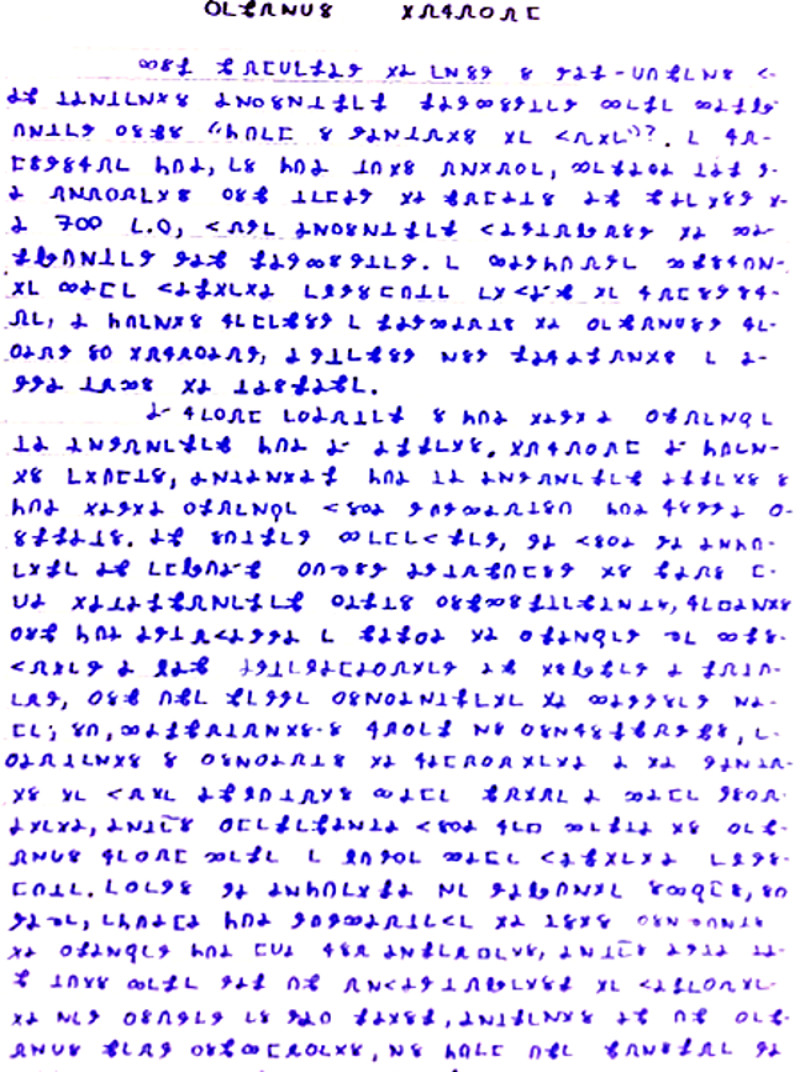
\includegraphics[width=.8\textwidth]{imagens/bruno.jpg}
  \caption{Texto criptografado pelo Menino do Acre}
  \label{fig:menino-do-acre}
\end{figure}

% Colocar aqui a frequência das letras em portugês, de preferência com um gráfico
% Inserir o exemplo do menino do Acre a partir do trabalho que eles enviarem
% Técnica para quebrar a cifra de Vigenère

